\section{Experiments}

\subsection{ImageNet classification}
\label{sec:imagenet}
We evaluate \mixup{} on the ImageNet-2012 classification dataset
\citep{ILSVRC15}. This dataset contains 1.3 million training images and 50,000
validation images, from a total of 1,000 classes. For training, we follow
standard data augmentation practices: scale and aspect ratio distortions,
random crops, and horizontal flips \citep{goyal2017accurate}. During
evaluation, only the $224\times 224$ central crop of each image is tested. We
use \mixup{} and ERM to train several state-of-the-art ImageNet-2012
classification models, and report both top-1 and top-5 error rates in
Table~\ref{table:imagenet_result}.

\begin{table}
	\centering
	\begin{tabular}[b]{ ll rrr }
		\toprule
		{Model} & {Method} & {Epochs} & {Top-1 Error} &  {Top-5 Error} \\
        \midrule
		{ResNet-50} & ERM \citep{goyal2017accurate} & $90$ & $23.5$ & {-} \\
		& \mixup{} $\alpha=0.2$ & $90$ & {$\bf 23.3$} &  {$\bf 6.6$}\\
		\cmidrule(lr){2-2}
		{ResNet-101} & ERM \citep{goyal2017accurate} & $90$ & $22.1$ & {-} \\
		& \mixup{} $\alpha=0.2$ & $90$ & {$\bf 21.5$} &  {$\bf 5.6$}\\
		\cmidrule(lr){2-2}
		{ResNeXt-101 32*4d} & ERM \citep{xie2016aggregated} & $100$ & $21.2$ & {-} \\
		& ERM & $90$ & $21.2$ & $5.6$ \\
		& \mixup{} $\alpha=0.4$ & $90$ & {$\bf 20.7$} &  {$\bf 5.3$}\\
		\cmidrule(lr){2-2}
        ResNeXt-101 64*4d  & ERM \citep{xie2016aggregated} & $100$ & $20.4$ & $5.3 $ \\
        & \mixup{} $\alpha=0.4$ & $90$ & {$\bf 19.8$} & {$\bf 4.9 $} \\
		\midrule
		{ResNet-50} & ERM & $200$ & $23.6$ & $7.0$ \\
		& \mixup{} $\alpha=0.2$ & $200$ & {$\bf 22.1$} &  {$\bf 6.1$}\\
		\cmidrule(lr){2-2}
		{ResNet-101} & ERM & $200$ & $22.0$ & $6.1$ \\
		 & \mixup{} $\alpha=0.2$ & $200$ & {$\bf 20.8$} &  {$\bf 5.4$}\\
		 \cmidrule(lr){2-2}
		{ResNeXt-101 32*4d}  & ERM & $200$ & $21.3$ & $5.9$ \\
		& \mixup{} $\alpha=0.4$ & $200$ & $\bf 20.1$ &  $\bf 5.0$\\
        \bottomrule
	\end{tabular}
    \caption{Validation errors for ERM and \mixup{} on the development set of
    ImageNet-2012.}
    \label{table:imagenet_result}
\end{table}

For all the experiments in this section, we use data-parallel distributed
training in Caffe2\footnote{\url{https://caffe2.ai}} with a minibatch size of 1,024. We use the learning rate schedule
described in \citep{goyal2017accurate}. Specifically, the learning rate is
increased linearly from 0.1 to 0.4 during the first 5 epochs, and it is then
divided by 10 after 30, 60 and 80 epochs when training for 90 epochs; or after
60, 120 and 180 epochs when training for 200 epochs.

For \mixup{}, we find that $\alpha \in [0.1, 0.4]$ leads to improved
performance over ERM, whereas for large $\alpha$, \mixup{} leads to
underfitting. We also find that models with higher capacities and/or longer
training runs are the ones to benefit the most from \mixup{}. For example, when
trained for 90 epochs, the \mixup{} variants of ResNet-101 and ResNeXt-101
obtain a greater improvement (0.5\% to 0.6\%) over their ERM analogues than the
gain of smaller models such as ResNet-50 (0.2\%). When trained for 200 epochs,
the top-1 error of the \mixup{} variant of ResNet-50 is further reduced by
1.2\% compared to the 90 epoch run, whereas its ERM analogue stays the same.

\subsection{CIFAR-10 and CIFAR-100}
\label{sec:cifar}
We conduct additional image classification experiments on the CIFAR-10 and
CIFAR-100 datasets to further evaluate the generalization performance of
\mixup{}. In particular, we compare ERM and \mixup{} training for: PreAct
ResNet-18 \citep{he2016identity} as implemented in \citep{cifar-pytorch},
WideResNet-28-10 \citep{Zagoruyko2016WRN} as implemented in
\citep{wide-sergey}, and DenseNet \citep{huang2017densely} as implemented in
\citep{dense-andreas}. For DenseNet, we change the growth rate to 40 to follow
the DenseNet-BC-190 specification from \citep{huang2017densely}.  For \mixup{},
we fix $\alpha=1$, which results in interpolations $\lambda$ uniformly
distributed between zero and one. All models are trained on a single Nvidia
Tesla P100 GPU using PyTorch\footnote{\url{http://pytorch.org}} for 200 epochs on the training set with 128 examples per
minibatch, and evaluated on the test set. Learning rates start at 0.1 and are
divided by 10 after 100 and 150 epochs for all models except WideResNet. For
WideResNet, we follow \citep{Zagoruyko2016WRN} and divide the learning rate by
10 after 60, 120 and 180 epochs. Weight decay is set to $10^{-4}$. We do not
use dropout in these experiments.

We summarize our results in Figure \ref{fig:cifar_results:table}. In both
CIFAR-10 and CIFAR-100 classification problems, the models trained using
\mixup{} significantly outperform their analogues trained with ERM. As seen in
Figure~\ref{fig:cifar_results:plot}, \mixup{} and ERM converge at a similar
speed to their best test errors.
%
Note that the DenseNet models in \citep{huang2017densely} were trained for 300
epochs with further learning rate decays scheduled at the 150 and 225 epochs,
which may explain the discrepancy the performance of DenseNet reported in
Figure \ref{fig:cifar_results:table} and the original result of
\citet{huang2017densely}.

\begin{figure}
	\centering
	\begin{subfigure}{0.6\textwidth}
		\centering
		\begin{tabular}[b]{ llrr }
            \toprule
			Dataset & Model & ERM &  \mixup{} \\
			\midrule
			\multirow{3}{*}{CIFAR-10} & PreAct ResNet-18 & $5.6$ &  $\bf 4.2$\\
			& WideResNet-28-10 & $3.8$ &  $\bf 2.7$\\
			& DenseNet-BC-190 & $3.7$ &  $\bf 2.7$\\
			\midrule
			\multirow{3}{*}{CIFAR-100} & PreAct ResNet-18 & $25.6$ &  $\bf 21.1$\\
			& WideResNet-28-10 & $19.4$ &  $\bf 17.5$\\
			& DenseNet-BC-190 & $19.0$ &  $\bf 16.8$\\
            \bottomrule
		\end{tabular}
        \caption{Test errors for the CIFAR experiments.}
        \label{fig:cifar_results:table}
	\end{subfigure}
	\hfill
	\begin{subfigure}{0.33\textwidth}
		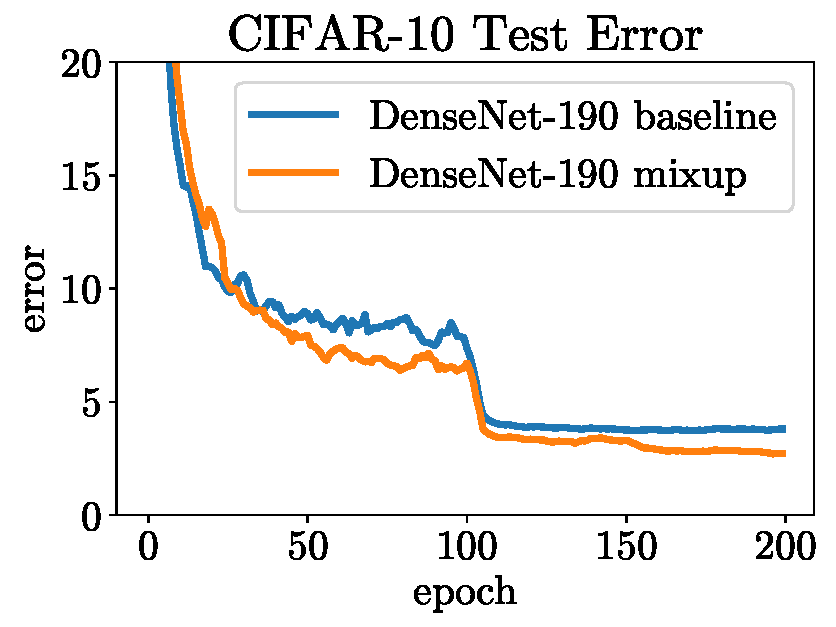
\includegraphics[width=\textwidth]{images/cifar10_test_error.pdf}
        \caption{Test error evolution for the best ERM and \mixup{} models.}
        \label{fig:cifar_results:plot}
	\end{subfigure}
    \caption{Test errors for ERM and \mixup{} on the CIFAR experiments.}
    \label{fig:cifar_results}
\end{figure}

\subsection{Speech data}
\label{sec:speech}
Next, we perform speech recognition experiments using the Google commands
dataset \citep{commands}. The dataset contains 65,000 utterances, where each
utterance is about one-second long and belongs to one out of 30 classes. The
classes correspond to voice commands such as \emph{yes, no, down, left}, as
pronounced by a few thousand different speakers. To preprocess the utterances,
we first extract normalized spectrograms from the original waveforms at a
sampling rate of 16 kHz. Next, we zero-pad the spectrograms to equalize their
sizes at $160 \times 101$. For speech data, it is reasonable to apply \mixup{}
both at the waveform and spectrogram levels. Here, we apply \mixup{} at the
spectrogram level just before feeding the data to the network.

For this experiment, we compare a LeNet \citep{lecun98} and a VGG-11
\citep{simonyan2014very} architecture, each of them composed by two
convolutional and two fully-connected layers. We train each model for 30 epochs
with minibatches of 100 examples, using Adam as the optimizer
\citep{kingma2014adam}. Training starts with a learning rate equal to
$3\times10^{-3}$ and is divided by 10 every 10 epochs.  For \mixup{}, we use a
warm-up period of five epochs where we train the network on original training
examples, since we find it speeds up initial convergence.
Table~\ref{fig:speech_results} shows that \mixup{} outperforms ERM on this
task, specially when using VGG-11, the model with larger capacity.

\begin{figure}
	\centering
		\begin{tabular}[b]{ll rr }
            \toprule
			Model & Method & Validation set & Test set\\
            \midrule
			\multirow{3}{*}{LeNet}  & ERM                     & $\bf 9.8$ & $\bf  10.3$\\
			                        & \mixup{} $(\alpha=0.1)$ &     $10.1$ &      $10.8$\\
			                        & \mixup{} $(\alpha=0.2)$ &    $10.2$ &      $11.3$\\
			\midrule
			\multirow{3}{*}{VGG-11} & ERM                     &     $5.0$ &      $4.6$\\
			                        & \mixup{} $(\alpha=0.1)$ &     $4.0$ &      $3.8$\\
			                        & \mixup{} $(\alpha=0.2)$ & $\bf 3.9$ &  $\bf 3.4$\\
            \bottomrule
		\end{tabular}
	\caption{Classification errors of ERM and \mixup{} on the Google commands dataset.}
    \label{fig:speech_results}
\end{figure}

\subsection{Memorization of corrupted labels}
\label{sec:corrupt}

Following \cite{2016arXiv161103530Z}, we evaluate the robustness of ERM and
\mixup{} models against randomly corrupted labels.  We hypothesize that
increasing the strength of \mixup{} interpolation $\alpha$ should generate
virtual examples further from the training examples, making memorization more
difficult to achieve.  In particular, it should be easier to learn
interpolations between real examples compared to memorizing interpolations
involving random labels. We adapt an open-source implementation
\citep{random-labels} to generate three CIFAR-10 training sets, where 20\%,
50\%, or 80\% of the labels are replaced by random noise, respectively. All the
test labels are kept intact for evaluation. Dropout
\citep{srivastava2014dropout} is considered the state-of-the-art method for
learning with corrupted labels \citep{arpit2017closer}. Thus, we compare in
these experiments \mixup{}, dropout, \mixup{} + dropout, and ERM. For \mixup{}, we choose $\alpha
\in \{1, 2, 8, 32\}$; for dropout, we add one dropout layer in each PreAct
block after the ReLU activation layer between two convolution layers, as
suggested in \citep{Zagoruyko2016WRN}. We choose the dropout probability $p \in
\{0.5, 0.7, 0.8, 0.9\}$. For the combination of \mixup{} and dropout, we choose $\alpha\in\{1, 2, 4, 8\}$ and $p\in\{0.3, 0.5, 0.7\}$. These experiments use the PreAct ResNet-18
\citep{he2016identity} model implemented in \citep{cifar-pytorch}. All the
other settings are the same as in Section \ref{sec:cifar}.

We summarize our results in Table \ref{table:corrupt}, where we note the best
test error achieved during the training session, as well as the final test
error after 200 epochs. To quantify the amount of memorization, we also
evaluate the training errors at the last epoch on real labels and corrupted
labels. As the training progresses with a smaller learning rate (e.g. less than
0.01), the ERM model starts to overfit the corrupted labels. When using a large
probability (e.g. 0.7 or 0.8), dropout can effectively reduce overfitting.
\mixup{} with a large $\alpha$ (e.g. 8 or 32) outperforms
dropout on both the best and last epoch test errors, and achieves lower
training error on real labels while remaining resistant to noisy labels. Interestingly, \mixup{} + dropout performs the best of all, showing that the two methods are compatible.

\begin{table}
  \centering
  \begin{tabular}[b]{ll rr rr}
    \toprule
    \multirow{2}{*}{Label corruption} & \multirow{2}{*}{Method} & \multicolumn{2}{c}{Test error} & \multicolumn{2}{c}{Training error} \\
    \cmidrule(lr){3-4} \cmidrule(lr){5-6}
    \rule{0pt}{2ex} & & Best & Last & Real & Corrupted \\
    \midrule
    \multirow{3}{*}{20\%} & ERM & $12.7$ & $16.6$ & $0.05$ & $0.28$ \\
    & ERM + dropout ($p=0.7$) & $8.8$ & $10.4$ & $5.26$ & $83.55$ \\
     & \mixup{} ($\alpha=8$)& $\bf 5.9$ & $6.4$ & $2.27$ & $86.32$ \\
    & \mixup{} + dropout ($\alpha=4, p=0.1$) & $6.2$ & $\bf 6.2$ & $1.92$ & $85.02$ \\
    \midrule
    \multirow{3}{*}{50\%} & ERM & $18.8$ & $44.6$ & $0.26$ & $0.64$ \\
    & ERM + dropout ($p=0.8$)& $14.1$ & $15.5$ & $12.71$ & $86.98$ \\
    & \mixup{} ($\alpha=32$) & $11.3$ & $12.7$ & $5.84$ & $85.71$ \\
    & \mixup{} + dropout ($\alpha=8, p=0.3$) & $\bf 10.9$ & $\bf 10.9$ & $7.56$ & $87.90$ \\
    \midrule
    \multirow{4}{*}{80\%} & ERM & $36.5$ & $73.9$ & $0.62$ & $0.83$ \\
    & ERM + dropout ($p=0.8$)& $30.9$ & $35.1$ & $29.84$ & $86.37$ \\
    & \mixup{} ($\alpha=32$) & $25.3$ & $30.9$ & $18.92$ & $85.44$ \\
    & \mixup{} + dropout ($\alpha=8, p=0.3$) & $\bf 24.0$ & $\bf 24.8$ & $19.70$ & $87.67$ \\
    \bottomrule
  \end{tabular}
  \caption{Results on the corrupted label experiments for the best models.}
  \label{table:corrupt}
\end{table}

\subsection{Robustness to Adversarial examples}
\label{sec:adversarial}

One undesirable consequence of models trained using ERM is their fragility to
adversarial examples~\citep{SzegedyZSBEGF13}. Adversarial examples are obtained
by adding tiny (visually imperceptible) perturbations to legitimate examples in
order to deteriorate the performance of the model.  The adversarial noise is
generated by ascending the gradient of the loss surface with respect to the
legitimate example. Improving the robustness to adversarial examples is a topic
of active research.

Among the several methods aiming to solve this problem,
some have proposed to penalize the norm of the Jacobian of the model to control
its Lipschitz constant~\citep{drucker1992improving, cisse2017parseval, bartlett2017spectrally,
hein2017formal}. Other approaches perform data augmentation by producing and
training on adversarial examples \citep{goodfellow2014explaining}.
Unfortunately, all of these methods add significant computational overhead to
ERM. Here, we show that
\mixup{} can significantly improve the robustness of neural networks without
hindering the speed of ERM by penalizing the norm of the gradient of the loss w.r.t a given input along the most plausible directions
(e.g. the directions to other training points). Indeed, Figure~\ref{fig:cifar10_interp} shows that \mixup{} results in models having a smaller loss and gradient norm between
examples compared to vanilla ERM.

To assess the robustness of \mixup{} models to adversarial examples, we use
three ResNet-101 models: two of them trained using ERM on ImageNet-2012, and
the third trained using \mixup{}. In the first set of experiments, we study the
robustness of one ERM model and the \mixup{} model against white box attacks.
That is, for each of the two models, we use the model itself to generate
adversarial examples, either using the Fast Gradient Sign Method (FGSM) or the
Iterative FGSM (I-FGSM) methods \citep{goodfellow2014explaining}, allowing a
maximum perturbation of $\epsilon=4$ for every pixel. For I-FGSM, we use 10
iterations with equal step size. In the second set of experiments, we evaluate
robustness against black box attacks. That is, we use the first ERM model to
produce adversarial examples using FGSM and I-FGSM. Then, we test the
robustness of the second ERM model and the \mixup{} model to these examples.
The results of both settings are summarized in Table~\ref{table:adversarial}.

For the FGSM white box attack, the \mixup{} model is $2.7$ times more robust
than the ERM model in terms of Top-1 error. For the FGSM black box attack, the
\mixup{} model is $1.25$ times more robust than the ERM model in terms of Top-1
error. Also, while both \mixup{} and ERM are not robust to white box I-FGSM
attacks, \mixup{} is about $40\%$ more robust than ERM in the black box I-FGSM
setting. Overall, \mixup{} produces neural networks that are significantly more
robust than ERM against adversarial examples in white box and black settings without additional overhead compared to ERM.

\begin{table}
  \begin{subfigure}{0.5\textwidth}
  \begin{center}
  \begin{tabular}[b]{ ll rr rr}
    \toprule
    Metric & Method & FGSM &  I-FGSM\\
    \midrule
    \multirow{2}{*}{Top-1} & ERM    & $    90.7$ & $99.9$\\
                           & \mixup & $\bf 75.2$ & $99.6$\\
    \midrule
    \multirow{2}{*}{Top-5} & ERM    &     $63.1$ & $93.4$\\
                           & \mixup & $\bf 49.1$ & $95.8$\\
    \bottomrule
  \end{tabular}
  \end{center}
  \caption{White box attacks.}
  \end{subfigure}
  \hfill
  \begin{subfigure}{0.5\textwidth}
  \begin{center}
  \begin{tabular}[b]{ ll rr}
    \toprule
    Metric & Method & FGSM &  I-FGSM \\
    \midrule
    \multirow{2}{*}{Top-1} & ERM    &     $57.0$ &     $57.3$\\
                           & \mixup & $\bf 46.0$ & $\bf 40.9$\\
    \midrule
    \multirow{2}{*}{Top-5} & ERM    &     $24.8$ &     $18.1$\\
                           & \mixup & $\bf 17.4$ & $\bf 11.8$\\
    \bottomrule
  \end{tabular}
  \end{center}
  \caption{Black box attacks.}
  \end{subfigure}
  \caption{Classification errors of ERM and \mixup{} models when tested on
  adversarial examples.}
  \label{table:adversarial}
\end{table}

\subsection{Tabular data}
\label{sec:uci}
To further explore the performance of \mixup{} on non-image data, we performed
a series of experiments on six arbitrary classification problems drawn from the
UCI dataset \citep{uci}. The neural networks in this section are
fully-connected, and have two hidden layers of 128 ReLU units. The parameters
of these neural networks are learned using Adam \citep{kingma2014adam}
with default hyper-parameters, over 10 epochs of mini-batches of size 16.
Table~\ref{table:uci} shows that \mixup{} improves the average test error on
four out of the six considered datasets, and never underperforms
ERM.

\begin{table}
  \begin{center}
  \begin{tabular}{ l r r}
  \toprule
  Dataset & ERM &  \mixup{} \\
  \midrule
  Abalone    & $74.0$  & $   73.6$ \\
  Arcene     & $57.6$  & $\bf 48.0$ \\
  Arrhythmia & $56.6$ & $\bf  46.3$\\
  \bottomrule
  \end{tabular}
  \hspace{0.8cm}
  \begin{tabular}{ l r r}
      \toprule
      Dataset & ERM &  \mixup{} \\
      \midrule
      Htru2    & $ 2.0$  & $    2.0$ \\
      Iris     & $21.3$ & $\bf 17.3$ \\
      Phishing & $16.3$ & $    15.2$ \\
      \bottomrule
  \end{tabular}
  \end{center}
  \caption{ERM and \mixup{} classification errors on the UCI datasets.}
  \label{table:uci}
\end{table}

\subsection{Stabilization of Generative Adversarial Networks (GANs)}
\label{sec:gans}

Generative Adversarial Networks, also known as GANs
\citep{goodfellow2014generative}, are a powerful family of implicit generative
models.  In GANs, a generator and a discriminator compete against each other to
model a distribution $P$. On the one hand, the generator $g$ competes to
transform noise vectors $z \sim Q$ into fake samples $g(z)$ that resemble real
samples $x \sim P$.  On the other hand, the discriminator competes to
distinguish between real samples $x$ and fake samples $g(z)$. Mathematically,
training a GAN is equivalent to solving the optimization problem
\begin{equation*}
  \max_g \min_d \E_{x, z} \, \ell(d(x), 1) + \ell(d(g(z)), 0),
\end{equation*}
where $\ell$ is the binary cross entropy loss. Unfortunately, solving the
previous min-max equation is a notoriously difficult optimization problem
\citep{goodfellow2016nips}, since the discriminator often provides the
generator with vanishing gradients.  We argue that \mixup{} should stabilize
GAN training because it acts as a regularizer on the gradients of the
discriminator, akin to the binary classifier in Figure~\ref{fig:mixup:toy}.
Then, the smoothness of the discriminator guarantees a stable source of
gradient information to the generator. The \mixup{} formulation of GANs is:
\begin{equation*}
  \max_g \min_d \E_{x, z, \lambda} \, \ell(d(\lambda x + (1 - \lambda) g(z)),
  \lambda).
\end{equation*}
Figure~\ref{fig:gans} illustrates the stabilizing effect of \mixup{} the
training of GAN (orange samples) when modeling two toy datasets (blue samples).
The neural networks in these experiments are fully-connected and have three
hidden layers of 512 ReLU units. The generator network accepts two-dimensional
Gaussian noise vectors. The networks are trained for 20,000 mini-batches of
size 128 using the Adam optimizer with default parameters, where the
discriminator is trained for five iterations before every generator iteration.
The training of \mixup{} GANs seems promisingly robust to hyper-parameter and
architectural choices.

\begin{figure}
    \begin{center}
    \resizebox{\textwidth}{!}{
    \begin{tabular}{c c}
        \toprule
        ERM GAN & \mixup{} GAN ($\alpha = 0.2$)\\
        \midrule
        \includegraphics[width=0.09\textwidth]{images/gan/{example_z=2_grid_0.0_000010}.png}
        \includegraphics[width=0.09\textwidth]{images/gan/{example_z=2_grid_0.0_000100}.png}
        \includegraphics[width=0.09\textwidth]{images/gan/{example_z=2_grid_0.0_001000}.png}
        \includegraphics[width=0.09\textwidth]{images/gan/{example_z=2_grid_0.0_010000}.png}
        \includegraphics[width=0.09\textwidth]{images/gan/{example_z=2_grid_0.0_020000}.png} &
        \includegraphics[width=0.09\textwidth]{images/gan/{example_z=2_grid_0.2_000010}.png}
        \includegraphics[width=0.09\textwidth]{images/gan/{example_z=2_grid_0.2_000100}.png}
        \includegraphics[width=0.09\textwidth]{images/gan/{example_z=2_grid_0.2_001000}.png}
        \includegraphics[width=0.09\textwidth]{images/gan/{example_z=2_grid_0.2_010000}.png}
        \includegraphics[width=0.09\textwidth]{images/gan/{example_z=2_grid_0.2_020000}.png}\\
        \includegraphics[width=0.09\textwidth]{images/gan/{example_z=2_ring_0.0_000010}.png}
        \includegraphics[width=0.09\textwidth]{images/gan/{example_z=2_ring_0.0_000100}.png}
        \includegraphics[width=0.09\textwidth]{images/gan/{example_z=2_ring_0.0_001000}.png}
        \includegraphics[width=0.09\textwidth]{images/gan/{example_z=2_ring_0.0_010000}.png}
        \includegraphics[width=0.09\textwidth]{images/gan/{example_z=2_ring_0.0_020000}.png}&
        \includegraphics[width=0.09\textwidth]{images/gan/{example_z=2_ring_0.2_000010}.png}
        \includegraphics[width=0.09\textwidth]{images/gan/{example_z=2_ring_0.2_000100}.png}
        \includegraphics[width=0.09\textwidth]{images/gan/{example_z=2_ring_0.2_001000}.png}
        \includegraphics[width=0.09\textwidth]{images/gan/{example_z=2_ring_0.2_010000}.png}
        \includegraphics[width=0.09\textwidth]{images/gan/{example_z=2_ring_0.2_020000}.png}\\
        \bottomrule
    \end{tabular}
    }
    \end{center}
    \caption{Effect of \mixup{} on stabilizing GAN training at iterations 10, 100, 1000, 10000, and 20000.}
    \label{fig:gans}
\end{figure}

\subsection{Ablation Studies}
\label{sec:ablation}
\mixup{} is a data augmentation method that consists of only two parts: random convex combination of raw inputs, and correspondingly, convex combination of one-hot label encodings. However, there are several design choices to make. For example, on how to augment the inputs, we could have chosen to interpolate the latent representations (i.e. feature maps) of a neural network, and we could have chosen to interpolate only between the nearest neighbors, or only between inputs of the same class. When the inputs to interpolate come from two different classes, we could have chosen to assign a single label to the synthetic input, for example using the label of the input that weights more in the convex combination. To compare \mixup{} with these alternative possibilities, we run a set of ablation study experiments using the PreAct ResNet-18 architecture on the CIFAR-10 dataset.

Specifically, for each of the data augmentation methods, we test two weight decay settings ($10^{-4}$ which works well for \mixup{}, and $5\times 10^{-4}$ which works well for ERM). All the other settings and hyperparameters are the same as reported in Section \ref{sec:cifar}.

\begin{table}
	\centering
	\begin{tabular}[b]{ll rr rr}
		\toprule
		\multirow{2}{*}{Method} & \multirow{2}{*}{Specification} & \multicolumn{2}{c}{Modified} & \multicolumn{2}{c}{Weight decay} \\
		\cmidrule(lr){3-4} \cmidrule(lr){5-6}
		\rule{0pt}{2ex} & & Input & Target & $10^{-4}$ & $5\times 10^{-4}$ \\
		\midrule
		ERM & & \xmark & \xmark & $5.53$ & $5.18$ \\
		\midrule
		\mixup{} & AC + RP & \cmark & \cmark &  $\bf 4.24$ & $4.68$ \\
		& AC + KNN & \cmark & \cmark & $4.98$ & $5.26$ \\
		\midrule
		mix labels and latent & Layer 1 & \cmark & \cmark & $4.44$ & $\bf 4.51$ \\
		representations & Layer 2 & \cmark & \cmark & $4.56$ & $4.61$ \\
		(AC + RP) & Layer 3 & \cmark & \cmark & $5.39$ & $5.55$ \\
		& Layer 4 & \cmark & \cmark & $5.95$ & $5.43$ \\
		& Layer 5 & \cmark & \cmark & $5.39$ & $5.15$ \\
		\midrule
		mix inputs only & SC + KNN \citep{chawla2002smote} & \cmark & \xmark & $5.45$ & $5.52$ \\
		& AC + KNN & \cmark & \xmark & $5.43$ & $5.48$ \\
		& SC + RP & \cmark & \xmark & $5.23$ & $5.55$ \\
		& AC + RP & \cmark & \xmark & $5.17$ & $5.72$ \\
		\midrule
		label smoothing & $\epsilon=0.05$ & \xmark & \cmark & $5.25$ & $5.02$ \\
		\citep{szegedy2016rethinking} & $\epsilon=0.1$ & \xmark & \cmark & $5.33$ & $5.17$ \\
		& $\epsilon=0.2$ & \xmark & \cmark & $5.34$ & $5.06$ \\
		\midrule
		mix inputs + & $\epsilon=0.05$ & \cmark & \cmark & $5.02$ & $5.40$ \\
		label smoothing & $\epsilon=0.1$ & \cmark & \cmark & $5.08$ & $5.09$ \\
		(AC + RP) & $\epsilon=0.2$ & \cmark & \cmark & $4.98$ & $5.06$ \\
		& $\epsilon=0.4$ & \cmark & \cmark & $5.25$ & $5.39$ \\
		\midrule
		add Gaussian noise & $\sigma=0.05$ & \cmark & \xmark & $5.53$ & $5.04$ \\
		to inputs & $\sigma=0.1$ & \cmark & \xmark & $6.41$ & $5.86$ \\
		& $\sigma=0.2$ & \cmark & \xmark & $7.16$ & $7.24$ \\
		\bottomrule
	\end{tabular}
	\caption{Results of the ablation studies on the CIFAR-10 dataset. Reported are the median test errors of the last 10 epochs. A tick (\cmark) means the component is different from standard ERM training, whereas a cross (\xmark) means it follows the standard training practice. AC: mix between all classes. SC: mix within the same class. RP: mix between random pairs. KNN: mix between k-nearest neighbors (k=200). Please refer to the text for details about the experiments and interpretations.}
	\label{table:ablation}
\end{table}

To compare interpolating raw inputs with interpolating latent representations, we test on random convex combination of the learned representations before each residual block (denoted Layer 1-4) or before the uppermost ``average pooling + fully connected" layer (denoted Layer 5). To compare mixing random pairs of inputs (RP) with mixing nearest neighbors (KNN), we first compute the 200 nearest neighbors for each training sample, either from the same class (SC) or from all the classes (AC). Then during training, for each sample in a minibatch, we replace the sample with a synthetic sample by convex combination with a random draw from its nearest neighbors. To compare mixing all the classes (AC) with mixing within the same class (SC), we convex combine a minibatch with a random permutation of its sample index, where the permutation is done in a per-batch basis (AC) or a per-class basis (SC). To compare mixing inputs and labels with mixing inputs only, we either use a convex combination of the two one-hot encodings as the target, or select the one-hot encoding of the closer training sample as the target. For label smoothing, we follow \cite{szegedy2016rethinking} and use $\frac{\epsilon}{10}$ as the target for incorrect classes, and $1-\frac{9\epsilon}{10}$ as the target for the correct class. Adding Gaussian noise to inputs is used as another baseline. We report the median test errors of the last 10 epochs. Results are shown in Table \ref{table:ablation}.

From the ablation study experiments, we have the following observations. First, \mixup{} is the best data augmentation method we test, and is significantly better than the second best method (mix input + label smoothing). Second, the effect of regularization can be seen by comparing the test error with a small weight decay ($10^{-4}$) with a large one ($5\times 10^{-4}$). For example, for ERM a large weight decay works better, whereas for \mixup{} a small weight decay is preferred, confirming its regularization effects. We also see an increasing advantage of large weight decay when interpolating in higher layers of latent representations, indicating decreasing strength of regularization.
Among all the input interpolation methods, mixing random pairs from all classes (AC + RP) has the strongest regularization effect. Label smoothing and adding Gaussian noise have a relatively small regularization effect. Finally, we note that the SMOTE algorithm \citep{chawla2002smote} does not lead to a noticeable gain in performance.
